\documentclass[12pt,]{article}


\usepackage{baskervillef}%polskie znaki może nie

%flow chatry
\usepackage{tikz}
\usetikzlibrary{shapes.geometric, arrows}
\usepackage{amssymb}
\usepackage{float}

\title{Sprawozadanie lernicng}
\author{Tymon Łazowy}
\date{123,2123,12}


\tikzstyle{startstop} = [ellipse, rounded corners, minimum width=2cm, minimum height=1cm,text centered, draw=black,thick,fill=red!0]

\tikzstyle{io} = [trapezium,
trapezium stretches=true,
trapezium left angle=70,
trapezium right angle=110,
thick,minimum width=2cm,
minimum height=0.85cm,
text centered,
draw=black,
fill=blue!0]

\tikzstyle{process} = [rectangle,
minimum width=3cm,
minimum height=0.85cm,
text centered,
text width=3cm,draw=black,thick,fill=orange!0]

\tikzstyle{decision} = [diamond,minimum width=1cm, minimum height=1cm, text centered, draw=black, fill=green!0,thick]

\tikzstyle{arrow} = [thick,->,>=stealth]

\begin{document}
 Równanie: $ax^2+bx+c=d$

D: a,b,c,d wyznaczniki $\in \mathbb R$ 

S: $x, x_0,x_1,x_2$ rozwiązanie równania $\in \mathbb{R}$ 
\begin{figure}[H]
   
    \caption{1.11 flowchart} 
    \centering  
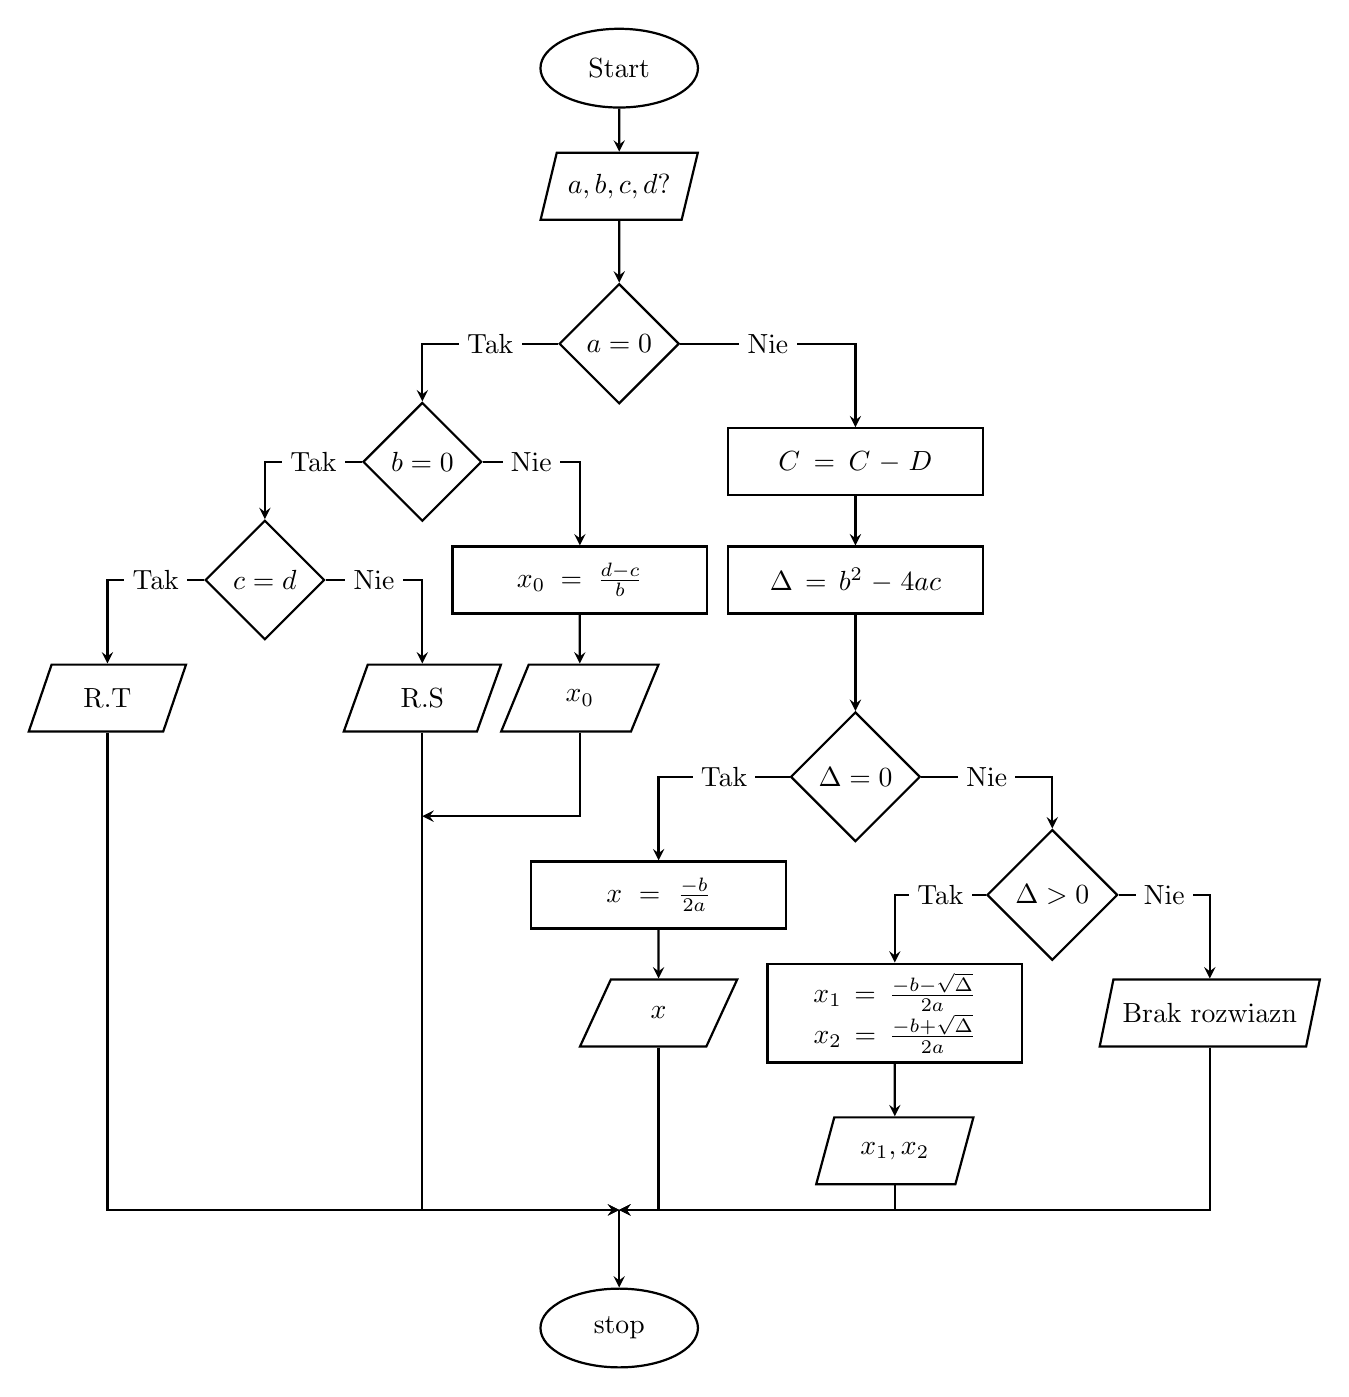
\begin{tikzpicture}[node distance=1.5cm]

\node (start) [startstop] {Start};
\node (in1) [io, below of=start] {$a,b,c,d ?$};

\node (dec) [decision, below of=in1,yshift=-0.5cm] {$a=0$};
%funkcja kwadratow
\node (nie) [process, right of=dec, xshift=1.5cm, yshift=-1.5cm] {$C=C-D$};
\node (pro2) [process, below of=nie] {$\Delta=b^2-4ac$};
\node (dec1) [decision, below of=pro2,yshift=-1.cm] {$\Delta=0$};
\node (tak1) [process, left of=dec1, xshift=-1.0cm, yshift=-1.5cm] {$x=\frac{-b}{2a}$};
\node (out1) [io, below of =tak1]{$x$};
\node (dec2) [decision, right of=dec1, xshift=1cm, yshift=-1.5cm] {$\Delta>0$};
\node (nie2) [io, right of=dec2, xshift=0.50cm, yshift=-1.5cm] {Brak rozwiazn};
\node (tak2) [process, left of=dec2, xshift=-0.50cm, yshift=-1.5cm] {$x_1=\frac{-b-\sqrt{\Delta}}{2a}$     $x_2=\frac{-b+\sqrt{\Delta}}{2a}$};
\node (out2) [io, below of =tak2,yshift=-0.25cm]{$x_1,x_2$};

\draw [arrow] (start) -- (in1);
\draw [arrow] (in1) -- (dec); 
\draw[arrow] (dec) -| (nie) node[pos=0.25,fill=white,inner sep=3]{Nie};
\draw [arrow] (nie) -- (pro2); 
\draw [arrow] (pro2) -- (dec1); 

\draw [arrow] (tak1) -- (out1);
\draw [arrow] (tak2) -- (out2);
\draw[arrow] (dec1) -| (dec2) node[pos=0.25,fill=white,inner sep=3]{Nie};
\draw[arrow] (dec1) -| (tak1) node[pos=0.25,fill=white,inner sep=3]{Tak};
\draw[arrow] (dec2) -| (tak2) node[pos=0.25,fill=white,inner sep=3]{Tak};
\draw[arrow] (dec2) -| (nie2) node[pos=0.25,fill=white,inner sep=3]{Nie};

%funkcja linowa
\node (1tak) [decision, left of =dec,xshift=-1.cm, yshift=-1.5cm]{$b=0$};
\node (2nie) [process, right of=1tak, xshift=0.5cm, yshift=-1.5cm] {$x_0=\frac{d-c}{b}$};
\node (1out) [io, below of =2nie]{$x_0$};
\node (2dec) [decision, left of=1tak, xshift=-0.50cm, yshift=-1.5cm] {$c=d$};
\node (3nie) [io, right of=2dec, xshift=0.50cm, yshift=-1.5cm] {R.S};
\node (3tak) [io, left of=2dec, xshift=-0.50cm, yshift=-1.5cm] {R.T};
\node (meeting)[coordinate,below of =start,yshift=-13cm]{};
\node (stop) [startstop, below of =meeting, yshift=0]{stop};
\node (mid)[coordinate,below of =3nie]{};

\draw[arrow] (dec) -| (1tak) node[pos=0.25,fill=white,inner sep=3]{Tak};
\draw[arrow] (1tak) -| (2dec) node[pos=0.25,fill=white,inner sep=3]{Tak};
\draw[arrow] (1tak) -| (2nie) node[pos=0.25,fill=white,inner sep=3]{Nie};
\draw[arrow] (2dec) -| (3tak) node[pos=0.25,fill=white,inner sep=3]{Tak};
\draw[arrow] (2dec) -| (3nie) node[pos=0.25,fill=white,inner sep=3]{Nie};
\draw [arrow] (2nie) -- (1out);
\draw [arrow] (3nie) |- (meeting);
\draw [arrow] (3tak) |- (meeting);
\draw [arrow] (1out) |- (mid);
\draw [arrow] (nie2) |- (meeting);
\draw [arrow] (out2) |- (meeting);
\draw [arrow] (out1) |- (meeting); 
\draw [arrow] (meeting)--(stop);
\end{tikzpicture}
    
    \label{flow11}
\end{figure}
\end{document}